% =====================================================================
% TikZ figure: 5-note example score on a treble staff (C4, E4, G4, A4, C5).
% Used as the running example throughout sections/04-math-foundations.tex.
% Pure black-and-white drawing without external glyphs.
% =====================================================================
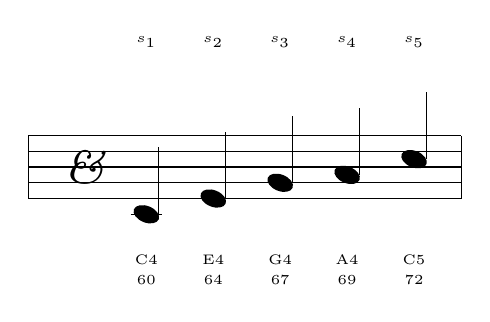
\begin{tikzpicture}[x=1mm,y=1mm,line width=0.4pt,font=\scriptsize]

  \def\stafflen{55}
  \def\noteh{1.4}
  % --- five horizontal lines of the treble staff ---
  \foreach \y in {0,2,4,6,8} \draw (0,\y) -- (\stafflen,\y);

  % --- bar lines ---
  \draw (0,0) -- (0,8);
  \draw (\stafflen,0) -- (\stafflen,8);

  % --- treble clef placeholder (simplified G-clef as text; not a real glyph) ---
  \node[anchor=west, scale=2.4] at (1.5, 4) {\textit{\&}};

  % --- note positions on the staff lines (treble clef):
  %   C4 = below the staff (1 ledger line below)
  %   E4 = bottom line          (y = 0)
  %   G4 = second line          (y = 2)
  %   A4 = second space         (y = 3)
  %   C5 = third space          (y = 5)
  % We place noteheads as filled ellipses; stems and labels below.
  \def\noteX{15} \def\noteSp{8.5}

  % helper: short ledger line for C4 below staff
  \draw (\noteX-2.0,-2) -- (\noteX+2.0,-2);

  \foreach \i/\xshift/\y/\name/\midi in {%
    1/0/-2/C4/60,
    2/1/0/E4/64,
    3/2/2/G4/67,
    4/3/3/A4/69,
    5/4/5/C5/72
  } {
    \pgfmathsetmacro{\xc}{\noteX + \xshift*\noteSp}
    % filled notehead (ellipse rotated)
    \begin{scope}[shift={(\xc,\y)},rotate=-22]
      \fill (0,0) ellipse (1.7 and 1.05);
    \end{scope}
    % stem upward
    \draw (\xc+1.6,\y) -- (\xc+1.6,\y+8.5);
    % label below
    \node[below=4mm,font=\tiny] at (\xc,-2) {\name};
    \node[below=6.5mm,font=\tiny] at (\xc,-2) {\midi};
  }

  % --- index labels above (i = 1..5) ---
  \foreach \i in {1,2,3,4,5} {
    \pgfmathsetmacro{\xc}{\noteX + (\i-1)*\noteSp}
    \node[above=10mm,font=\tiny] at (\xc,8) {$s_{\i}$};
  }

\end{tikzpicture}
